\subsection{Background and motivation}
Powered wheelchairs have substantially benefited people with mobility challenges.
The use of these wheelchair systems has been shown to improve the user's independence, quality
of life and feeling of well-being \cite{treflerOutcomesWheelchairSystems2004}.
However, this technology can be inaccessible or unsafe for people with vision impairment,
multiple sclerosis, ALS, and cerebral palsy, due to difficulties with environmental perception
or joystick use. A survey of 65 clinicians found that 10-40\% of patients found it impossible or
extremely difficult to use a powered wheelchair \cite{fehrAdequacyPowerWheelchair2000}.

Smart wheelchairs add intelligent sensing and control to an existing powered wheelchair
to avoid obstacles in the environment or to navigate the user.
A smart wheelchair may include alternative input methods such as
eye gaze \cite{eidNovelEyeGazeControlledWheelchair2016}, head tilt \cite{tomariEnhancingWheelchairControl2014},
and voice recognition \cite{bakouriSteeringRoboticWheelchair2022}.
Fully-autonomous smart wheelchairs move the user from a start pose to an end goal,
and often require a map of the surrounding environment or markers
such as QR codes \cite{habhaAutonomousWheelchairIndoorOutdoor2021}.
Semi-autonomous smart wheelchairs blend input from the user with the control unit
to avoid obstacles and improve safety. Using a smart wheelchair improves the user's
safety and independence; Simpson et al. found that over 61\% of
current wheelchair users would benefit from some smart wheelchair features \cite{simpsonHowManyPeople2008}.

\subsection{Aims}
This research aims to develop a semi-autonomous smart wheelchair system.
This research was done in collaboration with Glide, a WA wheelchair manufacturer,
who has provided an existing powered wheelchair (CentroGlide) to use as a base
for this functionality (\cref{fig:wheelchair}). By developing assistive technology for the wheelchair,
the user is granted greater mobility, confidence, and independence.

The project team comprises multiple engineering project students, researchers, and interns.
This team has worked on many smart wheelchair features, including motor controller design (Kosma Egan),
input controller design (Brian Smith), doorway navigation (Avinash Sudhakaran),
object detection (Krishnadas Suresh), and navigation to a vehicle (Nicolas Lee).
The specific aim of this thesis is to implement navigation assistance,
which involves both avoiding environmental obstacles such as walls and stairs,
and guiding the user along suitable pathways. If a user were to unintentionally
drive off a pathway, they could encounter a kerb or uneven terrain, which could lead
to a fall.

\pagebreak
\subsection{Problem definition}
An important requirement of this system is that the user still
has control over their wheelchair and can override any autonomous functionality
if required. If the smart wheelchair system mistakenly detects an obstacle,
the user's mobility should not be compromised.

Another requirement of the system is that any sensors mounted to the wheelchair
should not impede the user's comfort or the wheelchair's manoeuvrability.
Many wheelchair users have specific requirements for wheelchair seat adjustments
to avoid pressure sores and discomfort. \Cref{fig:wheelchair} shows the
wheelchair configuration when fully reclined, demonstrating that some sensor mounting locations
are infeasible.

The smart wheelchair system should also be commercially viable - high-cost
components and sensors are infeasible. Internet connectivity should not be a requirement
for the system to operate either - the round trip time required to communicate with a server
could compromise the safety of a user. Because of this, all processing is performed locally
on the wheelchair.

\begin{figure}[b]
    \centering
    \begin{subfigure}{.45\textwidth}
        \centering
        \includegraphics[height=\linewidth,angle=270,origin=c]{images/wheelchair.jpg}
        \caption{Upright}
    \end{subfigure}
    \quad
    \begin{subfigure}{.45\textwidth}
        \centering
        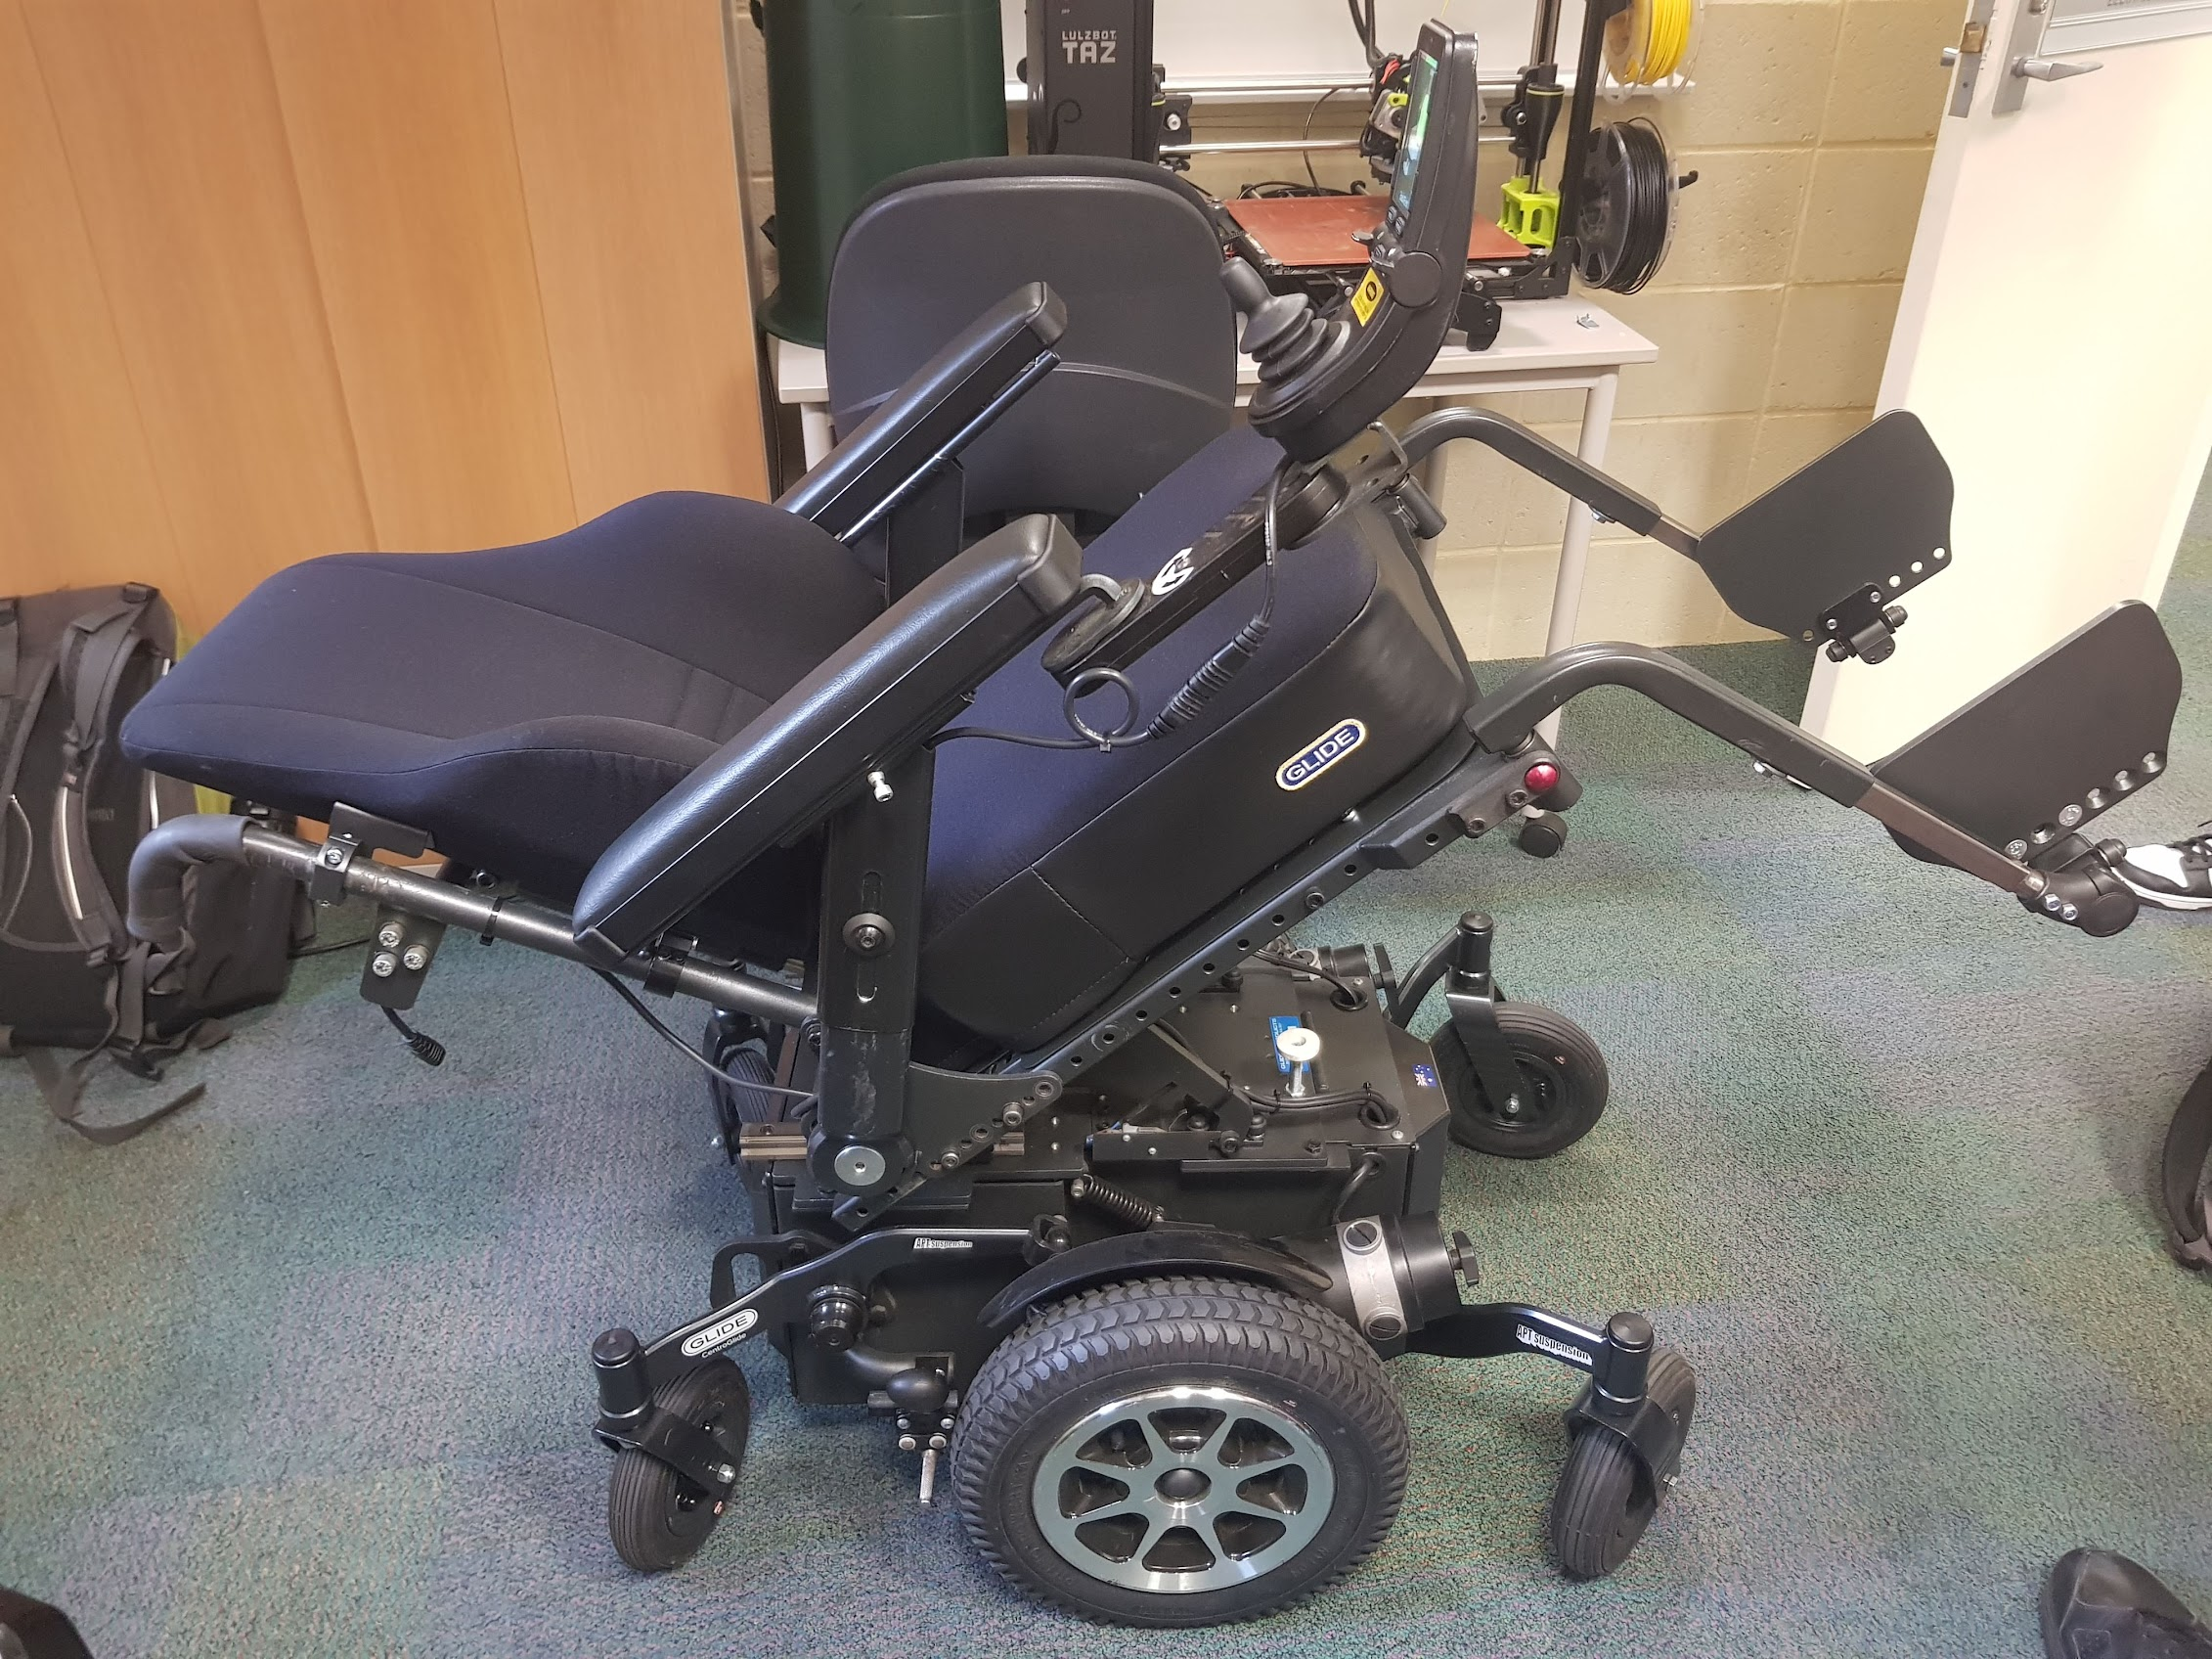
\includegraphics[width=\linewidth]{images/wheelchair_reclined.jpg}
        \caption{Reclined}
    \end{subfigure}
    \caption{CentroGlide wheelchair}
    \label{fig:wheelchair}
\end{figure}
